\documentclass[ignorenonframetext]{beamer}

\title{Learning to map strings to meaning}
\subtitle{Comp 542 Natural Language Processing}
\author{Deniz Yuret}
%\date{Comp 542, Fall 2013}

\hypersetup{colorlinks,urlcolor=red}

\begin{document}

\begin{frame}
\maketitle
\end{frame}

\begin{frame}\frametitle{SHRDLU}

\begin{itemize}
\item Domain: blocks in a virtual world
\item Input: user commands and questions
\item Output: appropriate answers and actions
\item Learning: none, manually built
\end{itemize}

See \href{http://hci.stanford.edu/~winograd/shrdlu}{Winograd, 1971}
and click on the following image for a demo.

\begin{center}
\href{http://youtu.be/QAJz4YKUwqw}{
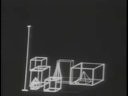
\includegraphics[]{images/winograd-shrdlu.png}}
\end{center}

\end{frame}

\begin{frame}\frametitle{SHRDLU: example interaction}
\begin{itemize}
\item pick up a big red block. 
\\ {\sl ok. (does it) }
\item grasp the pyramid. 
\\ {\sl i don't understand which pyramid you mean. }
\item find a block which is taller than the one you are holding and put it into the box. 
\\ {\sl by ``it'', i assume you mean the block which is taller than the one i am holding.  ok. (does it) }
\item what does the box contain? 
\\ {\sl the blue pyramid and the blue block. }
\item what is the pyramid supported by? 
\\ {\sl the box. }
\item how many blocks are not in the box? 
\\ {\sl four of them. }
\item is at least one of them narrower than the one which i told you to pick up? 
\\ {\sl yes, the red cube. }
%% \item is it supported? 
%% \\ {\sl yes, by the table. }
%% \item can the table pick up blocks? 
%% \\ {\sl no. }
%% \item can a pyramid be supported by a block? 
%% \\ {\sl yes. }
%% \item can a pyramid support a pyramid? 
%% \\ {\sl i don't know. }
%% \item stack up two pyramids. 
%% \\ {\sl i can't. }
\end{itemize}
\end{frame}

\begin{frame}\frametitle{SHRDLU maps sentences to procedures}
A command like
\begin{quote}
Put a red pyramid on top of the blue block
\end{quote}
gets mapped to a procedure that uses three basic actions
\begin{itemize}
\item MOVETO(a location)
\item GRASP(a block)
\item UNGRASP(a block)
\end{itemize}
\end{frame}

\begin{frame}\frametitle{SHRDLU maps sentences to procedures}
\begin{quote}
Put a red pyramid on top of the blue block
\end{quote}

The ``put'' command corresponds to an UNGRASP action if the following satisfied:
\begin{itemize}
\item the blue block has nothing on top
\item the robot hand is holding the red pyramid
\item it is on top of the blue block
\end{itemize}
If not SHRDLU searches for possible actions to satisfy them.
\vspace*{1em}

\color{red} 
Note that the resulting procedure depends on both the sentence
and the current state of the world.
\end{frame}

\begin{frame}\frametitle{START}

\begin{itemize}
\item Domain: simplified text, structured websites
\item Input: user questions
\item Output: appropriate answers
\item Learning: none, manually built
\end{itemize}

See \href{ftp://publications.ai.mit.edu/ai-publications/pdf/AIM-1096.pdf}{Katz, 1988}
and click on the following image for a demo.

\begin{center}
\href{http://start.csail.mit.edu}{
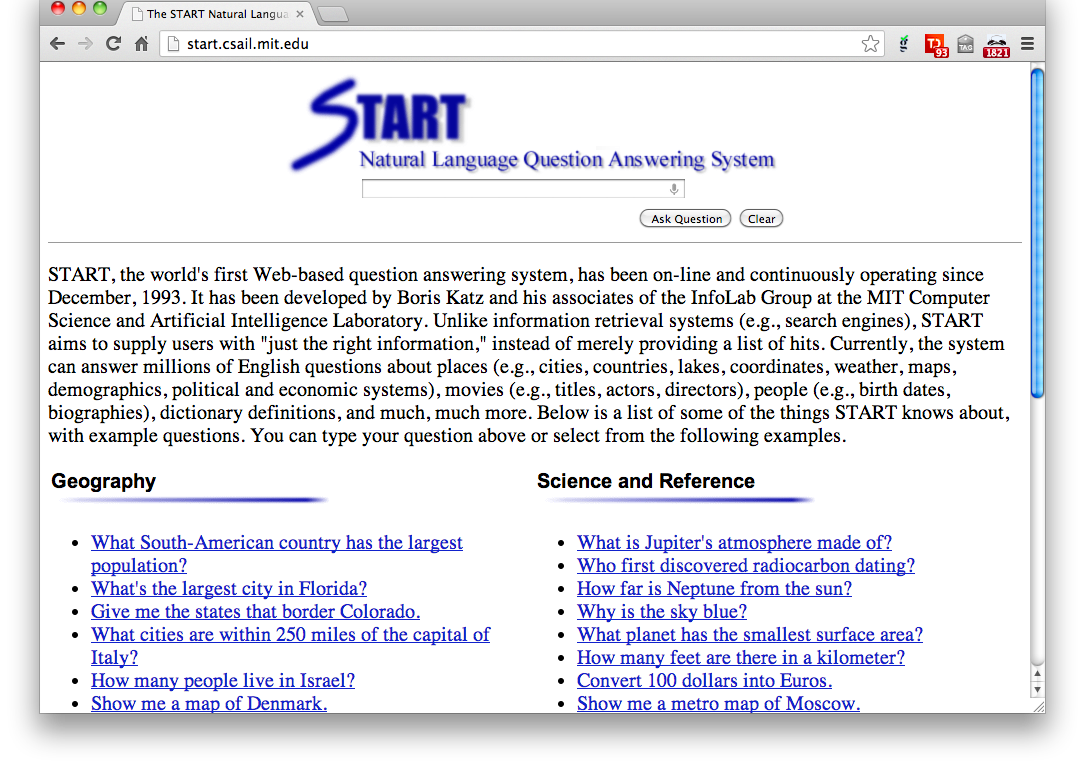
\includegraphics[width=.7\textwidth]{images/katz-start.png}}
\end{center}

\end{frame}

\begin{frame}\frametitle{START: example questions}
{\bf Geography}\begin{itemize}
\item What South-American country has the largest population?
\item What's the largest city in Florida?
\end{itemize}

{\bf Science and Reference}\begin{itemize}
\item What is Jupiter's atmosphere made of?
\item Who first discovered radiocarbon dating?
\end{itemize}

{\bf Arts and Entertainment}\begin{itemize}
\item Who directed Gone with the Wind?
\item Show some paintings by Claude Monet.
\end{itemize}

{\bf History and Culture}\begin{itemize}
\item What countries speak Spanish?
\item Who was president in 1881?
\end{itemize}
\end{frame}

\begin{frame}\frametitle{START maps sentences to T-expressions}
A T-expression (ternary expression) is a 
\begin{quote}
$\langle${\bf subject relation object}$\rangle$ triple.
\end{quote}
A complex sentence such as:
\begin{quote}
If the orator wants to persuade people, he must speak the things
people wish to hear.
\end{quote}
is broken down into the following units (kernel sentences) and stored as T-expressions:
\begin{itemize}
\item[(S1)] $\langle${\bf orator-1 want S2}$\rangle$
\item[(S2)] $\langle${\bf orator-1 persuade people-2}$\rangle$
\item[(S3)] $\langle${\bf he-1 speak things-3}$\rangle$
\item[(S4)] $\langle${\bf people-2 wish S5}$\rangle$
\item[(S5)] $\langle${\bf people-2 hear things-3}$\rangle$
\end{itemize}
\end{frame}

\begin{frame}\frametitle{START maps sentences to T-expressions}
\begin{itemize}
\item T-expressions are generated and indexed upon reading text.
\item T-expressions are matched when the user asks a question.
\item S-rules (S stands for both syntax and semantics) handle paraphrases:
\begin{quote}
Miriam presented Gabriela with a gift.\\
Miriam presented a gift to Gabriela.
\end{quote}
\item OmniBase annotates multimedia and structured websites (IMDB,
  World Factbook, Wikipedia) with simple English to support matching
  and retrieval from the web.  See
  (\href{http://www.denizyuret.com/pub/nldb02/Katz-etal-NLDB02.pdf}{Katz,
    Felshin, Yuret et al. 2002}) for more information.
\vspace*{1em}

{\small\sl
(get "imdb-movie" "Gone with the Wind (1939)" "DIRECTOR") 
\\ =$>$ ("George Cukor" "Victor Fleming" "Sam Wood")
}
\end{itemize}
\end{frame}

\begin{frame}\frametitle{GEOQUERY}

\begin{itemize}
\item Domain: US Geography Database
\item Input: user questions
\item Output: appropriate answers
\item Learning: from question, logical form pairs
\end{itemize}

See \href{http://aaaipress.org/Papers/AAAI/1996/AAAI96-156.pdf}{Zelle
  and Mooney, 1996}
and click on the following image for more information.

\begin{center}
\href{http://www.cs.utexas.edu/users/ml/geo.html}{
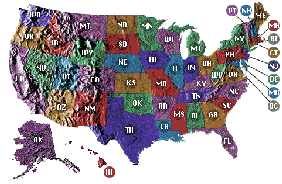
\includegraphics[width=.7\textwidth]{images/us-states.png}}
\end{center}

\end{frame}

\begin{frame}\frametitle{GEOQUERY: database}
A small database with about 800 facts on US geography:
\begin{itemize}
\item States - their capitals, populations, areas, population densities,
major cities, rivers and the bordering states
\item Cities - their populations and the states they are in
\item Rivers - their lengths and the states through which they flow
\item Mountains - their heights and the states they are in
\end{itemize}
\vspace*{1cm}
Note: Other databases commonly used in semantic parsing literature in addition to
\href{http://www.cs.utexas.edu/users/ml/nldata/geo.html}{\sc geoquery} include
\href{http://www.cs.utexas.edu/users/ml/nldata/restquery.html}{\sc rest} (restaurant information in N. California),
\href{http://www.cs.utexas.edu/users/ml/nldata/jobquery.html}{\sc jobs} (job announcements from austin.jobs),
\href{http://www.cs.utexas.edu/users/ml/nldata/clang.html}{\sc clang} (the RoboCup coach language).
\end{frame}

\begin{frame}\frametitle{GEOQUERY: example questions}
\begin{itemize}
\item What is the capital of Texas?
\item What is the length of Colorado?
\item What is the population of Colorado?
\item What is the area of the largest state?
\item What are the major cities in Louisiana?
\item How many people live in South Dakota?
\item How high is the highest point in Alaska?
\item Which states have a city named Springfield?
\item What is the capital of the most populous state?
\item How many rivers flow through Mississippi?
\item How many states does the Mississippi run through?
\item How high is the highest point in the smallest state?
\item Which rivers flow through the states that border California?
\end{itemize}
\end{frame}

\begin{frame}\frametitle{GEOQUERY: learning to map questions to logical forms}
Example: What states border Montana?
\begin{itemize}
%% \item syntax: \\
%% {\tt (SBARQ (WHNP (WP What) (NNS states)) \\ \hspace{8ex} (SQ (VP (VBP border) (NP (NNP Montana)))))}
\item Prolog:
(\href{http://aaaipress.org/Papers/AAAI/1996/AAAI96-156.pdf}{Zelle and Mooney 1996}; 
 \href{}{Tang and Mooney 2001})
\\ {\tt \small answer(A,(state(A),next-to(A,B),const(B,stateid(montana))))}
\item SQL:
(\href{http://homes.cs.washington.edu/~etzioni/papers/nli-iui03.pdf}{Popescu et al. 2003};
 \href{https://forum.disi.unitn.it/~moschitt/articles/NLDB09.pdf}{Giordani and Moschitti 2010})
\\ {\tt SELECT state1 FROM borders WHERE state2='montana'}
\item FunQL: 
(\href{}{Kate, Wong, and Mooney 2005})
\\ {\tt answer(state(next-to-2(stateid('montana'))))}
\item Lambda calculus: 
(\href{}{Zettlemoyer and Collins 2005})
\\ {\tt $\lambda$x.state(x)$\land$borders(x,montana)}
\end{itemize}
\end{frame}

\begin{frame}\frametitle{GEOQUERY: learning with indirect supervision}
\begin{itemize}
\item Kate and Mooney 2007 learn from multiple potential meaning representations, only one of which is correct.
\end{itemize}
\end{frame}

\begin{frame}\frametitle{NAVIGATION}
MacMahon 2006
Zettlemoyer 2013
Mooney 2011
\end{frame}

\begin{frame}\frametitle{MAPTASK}
HCRC Map Task Corpus (Anderson et al. 1991)
Vogel and Jurafsky, 2010

\end{frame}


\begin{frame}\frametitle{SPORTSCASTER}

\begin{itemize}
\item Domain: RoboCup soccer games
\item Input: game state
\item Output: game commentary
\item Learning: from sample commentaries
\end{itemize}

See \href{http://www.cs.utexas.edu/~ai-lab/pub-view.php?PubID=126770}{Chen and Mooney, 2008} 
and \href{http://cs.stanford.edu/~pliang/papers}{Liang, Jordan, and Klein, 2009}
for more information.

\begin{center}
\href{http://www.cs.utexas.edu/~ai-lab/pub-view.php?PubID=126770}{
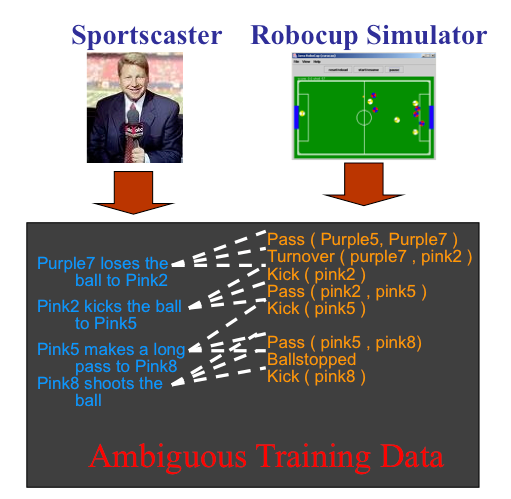
\includegraphics[height=.7\textheight]{images/chen-sportscast.png}}
\end{center}
\end{frame}

\begin{frame}\frametitle{Learning to map video to language}
\begin{itemize}
\item Domain: human physical actions
\item Input: video
\item Output: verbal description
\item Learning: none, manually built
\end{itemize}

\begin{center}
\href{http://groups.csail.mit.edu/genesis/movies/redandbluemen.mp4}{
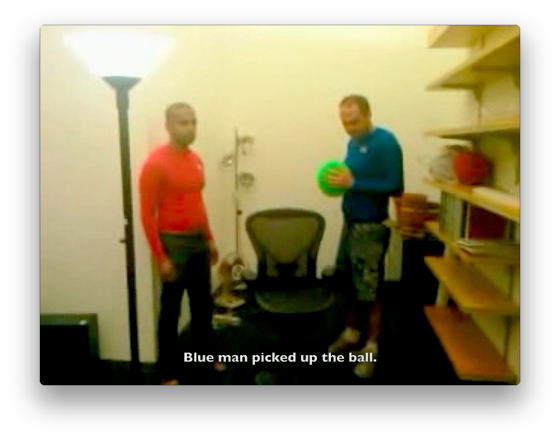
\includegraphics[height=.7\textheight]{images/redandbluemen.png}}
\end{center}
\end{frame}

\begin{frame}\frametitle{Learning to map video to language}
\begin{center}
More vision demonstrations from the MIT Genesis Group:
\vspace{1em}

\href{http://groups.csail.mit.edu/genesis/visiondemonstrations}{
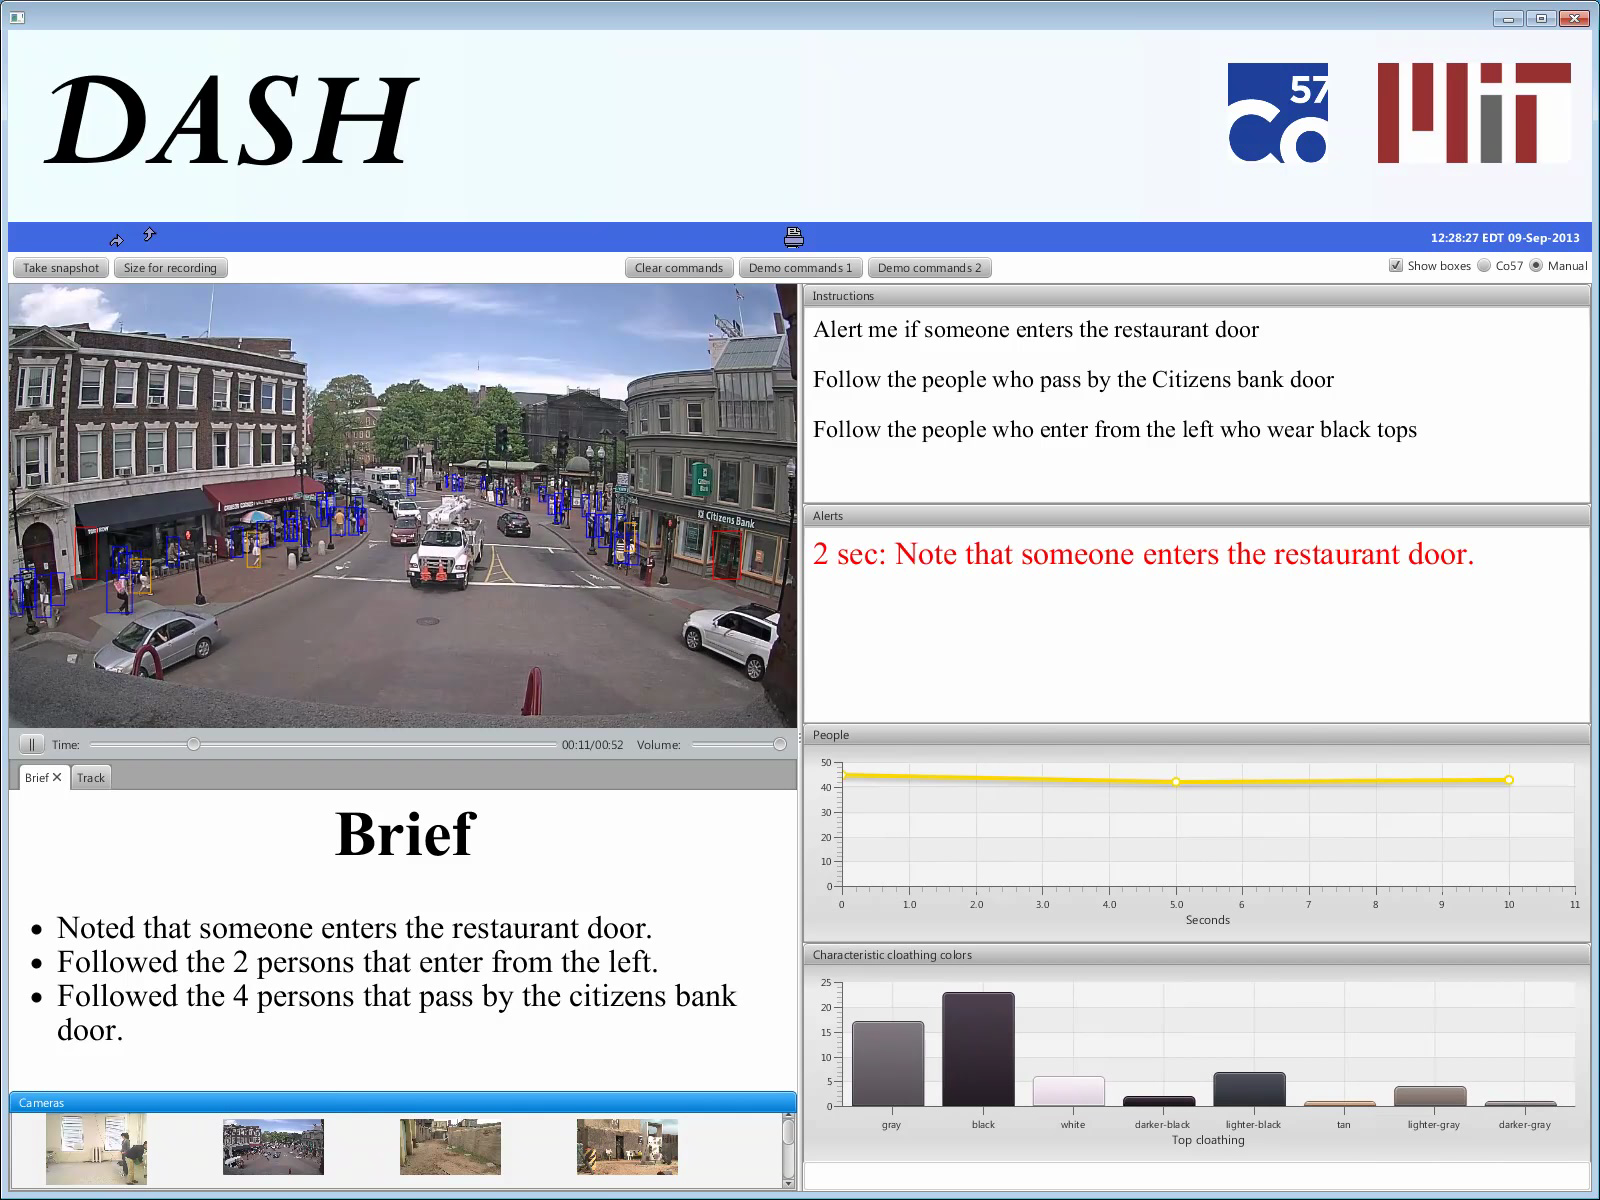
\includegraphics[height=.7\textheight]{images/genesis-vision.png}}
\end{center}
\end{frame}

\begin{frame}\frametitle{Reinforcement learning for mapping instructions to actions}
\begin{itemize}
\item Domain: Windows PC interface, puzzles, games
\item Input: Help documents
\item Output: User action sequence
\item Learning: Reinforcement learning via reward signal
\end{itemize}
See \href{http://groups.csail.mit.edu/rbg/code/rl}{Branavan et al. 2009},
\href{http://groups.csail.mit.edu/rbg/code/rl-hli}{2010},
\href{http://groups.csail.mit.edu/rbg/code/civ}{2011}, and
\href{http://people.csail.mit.edu/branavan}{Branavan's thesis}
for more information.
\begin{center}
\href{http://groups.csail.mit.edu/rbg/code/civ}{
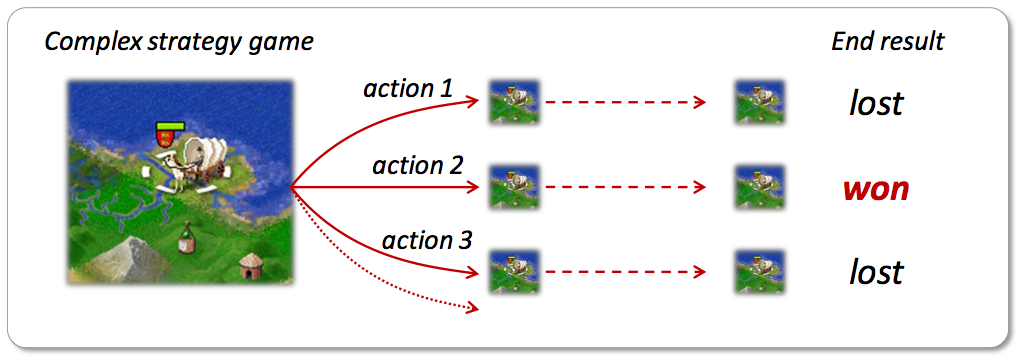
\includegraphics[width=\textwidth]{images/branavan-civ2.png}}
\end{center}
\end{frame}

\begin{frame}\frametitle{Reinforcement learning for mapping instructions to actions}
\begin{center}
\href{http://groups.csail.mit.edu/rbg/code/rl}{
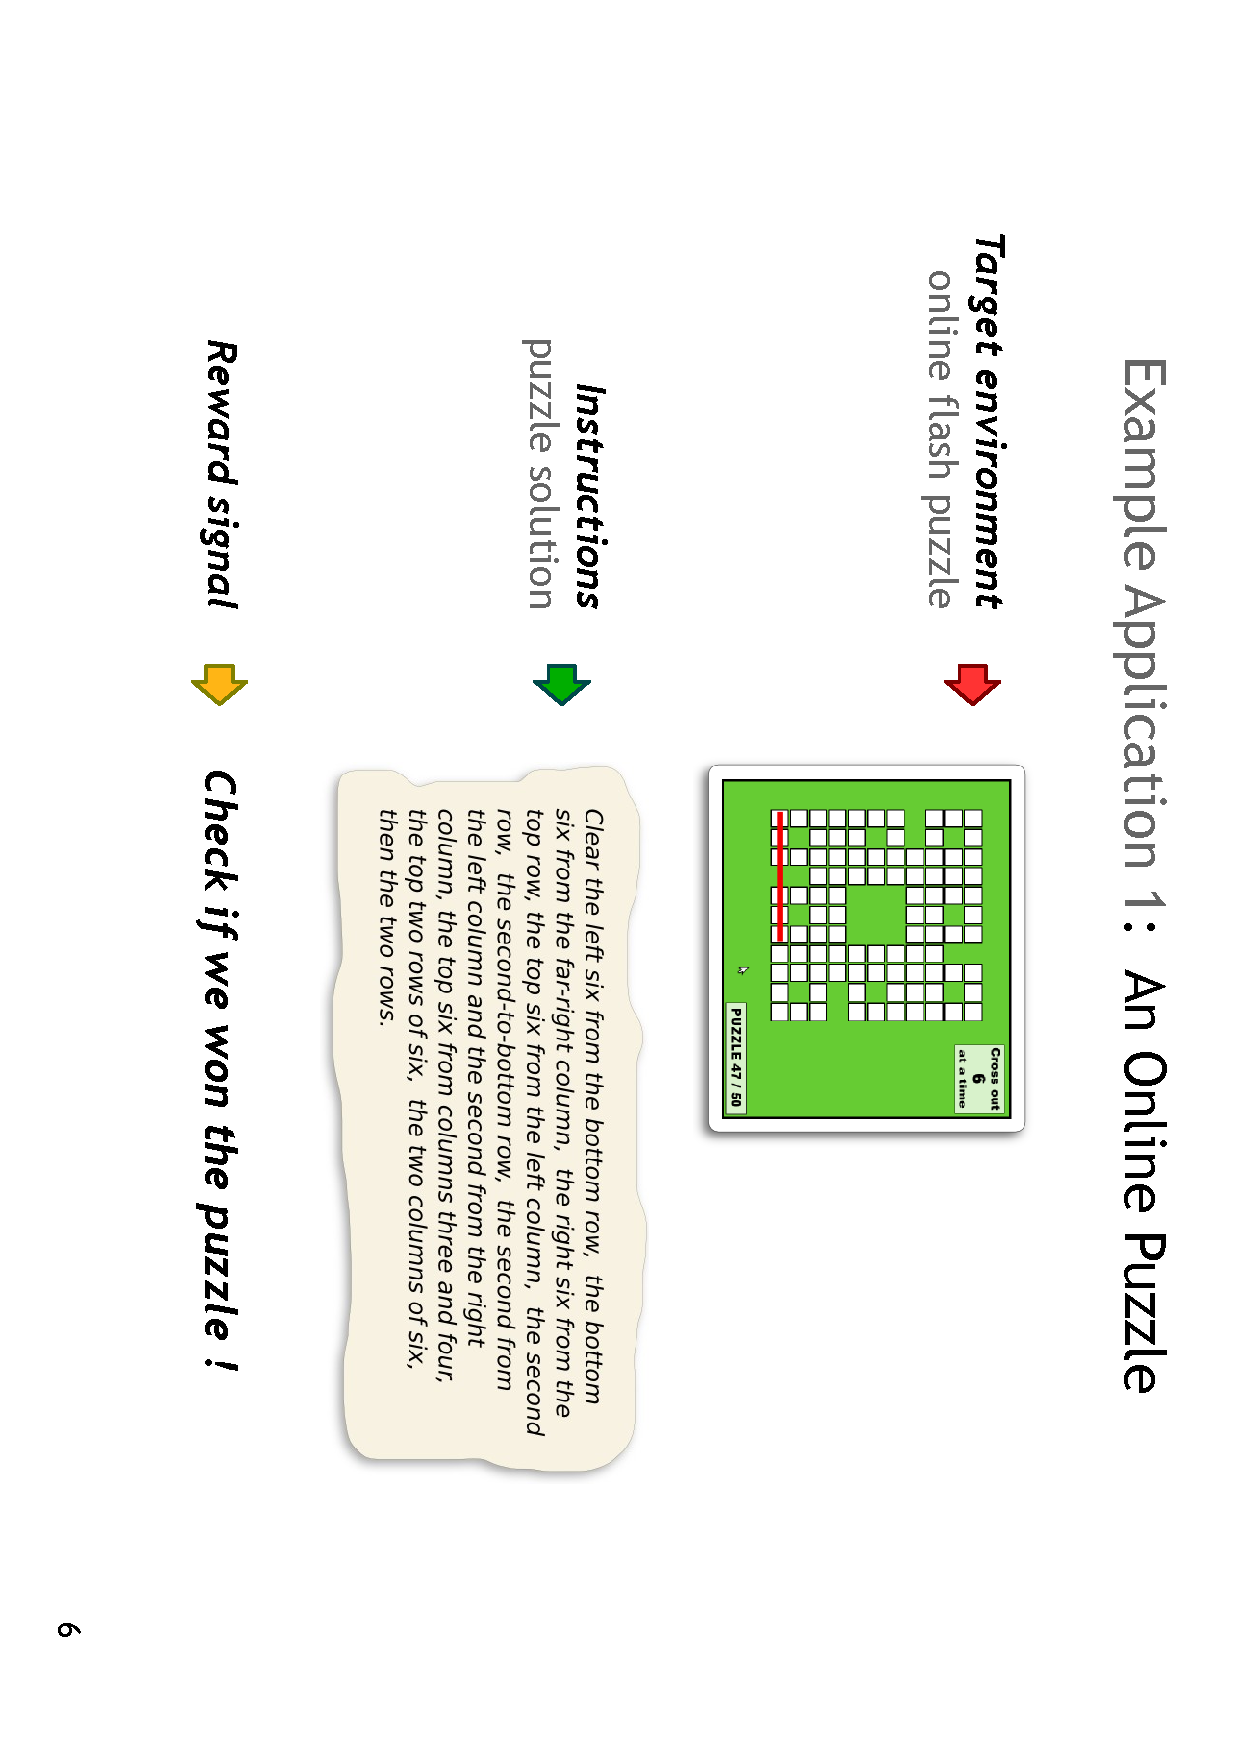
\includegraphics[angle=90,width=\textwidth]{images/branavan-crossblock.pdf}}
\end{center}
\end{frame}

\begin{frame}\frametitle{Reinforcement learning for mapping instructions to actions}
\begin{center}
\href{http://groups.csail.mit.edu/rbg/code/rl-hli}{
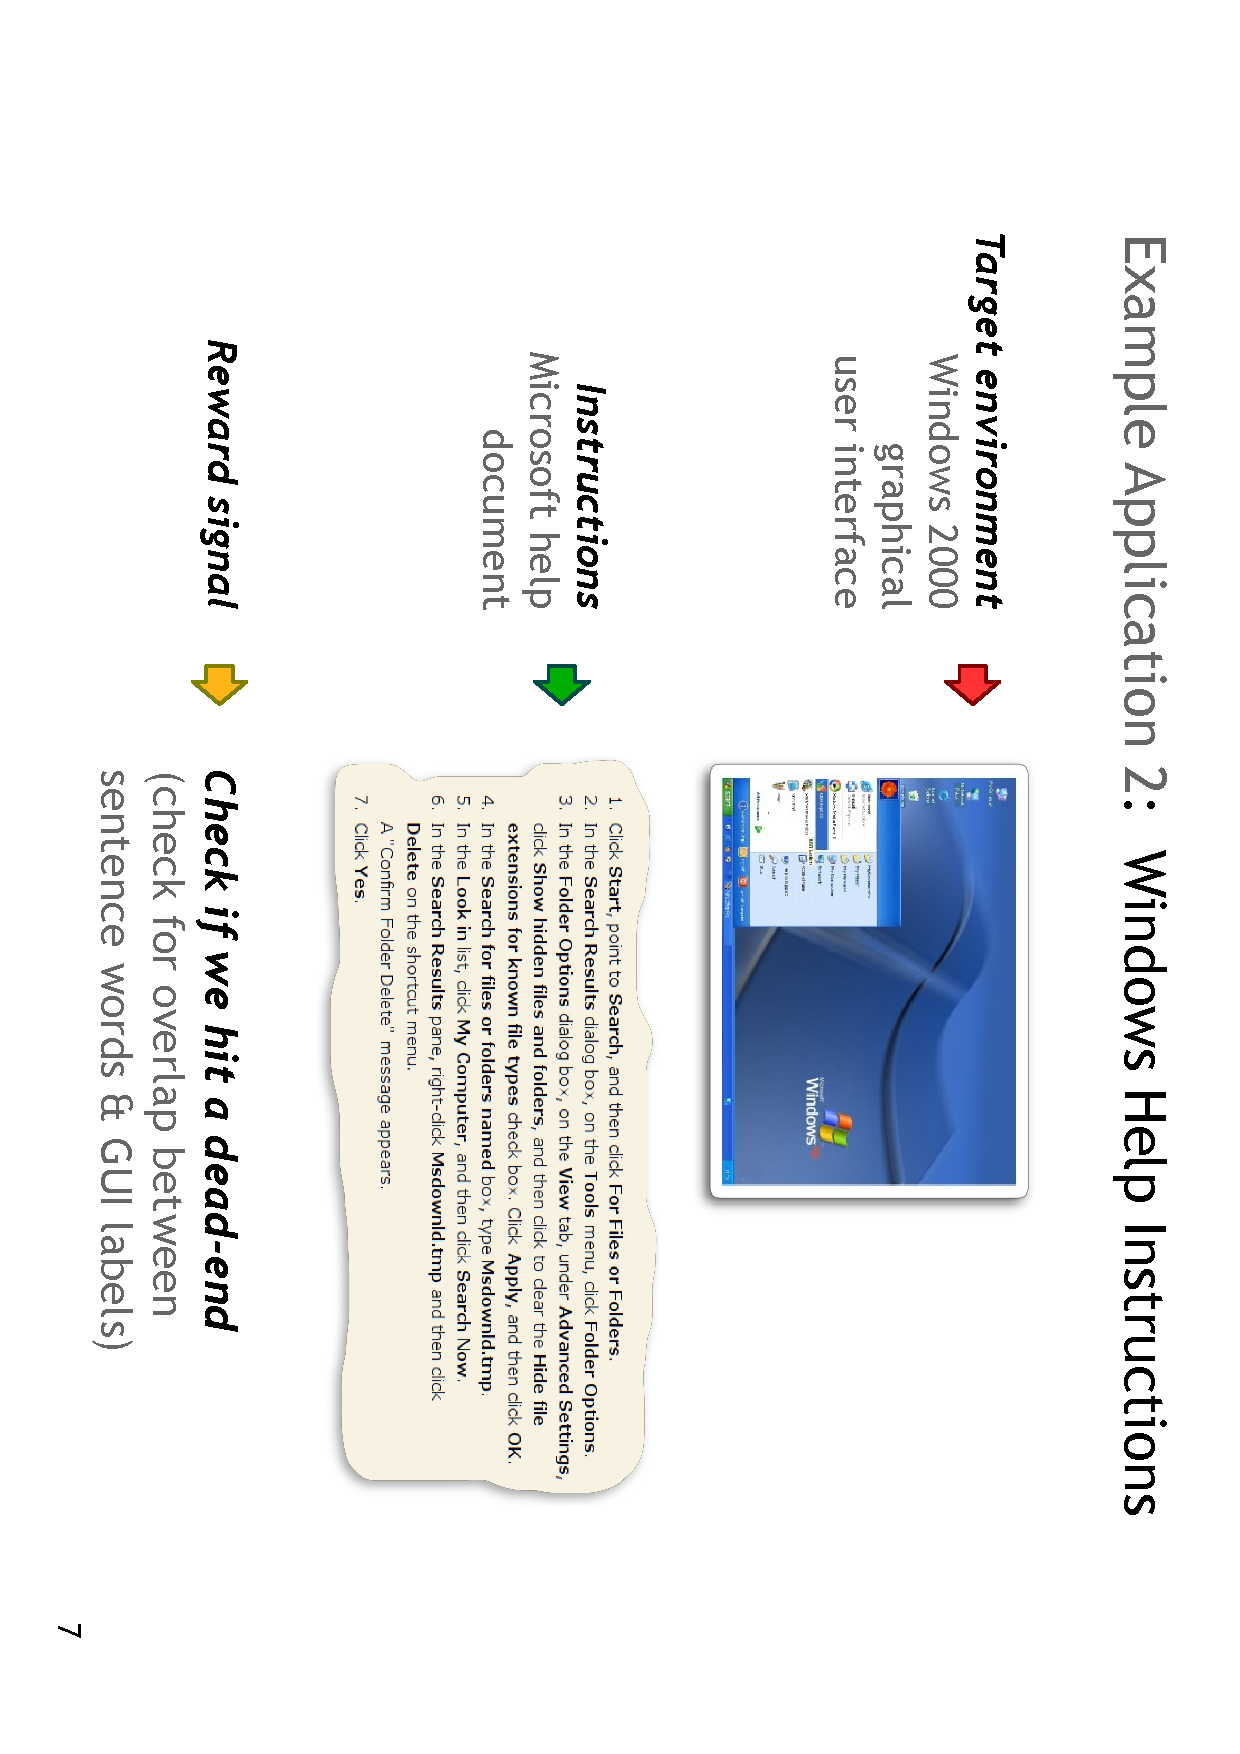
\includegraphics[angle=90,width=\textwidth]{images/branavan-windows.pdf}}
\end{center}
\end{frame}

\begin{frame}\frametitle{Reinforcement learning for mapping instructions to actions}
\begin{center}
\href{http://groups.csail.mit.edu/rbg/code/civ}{
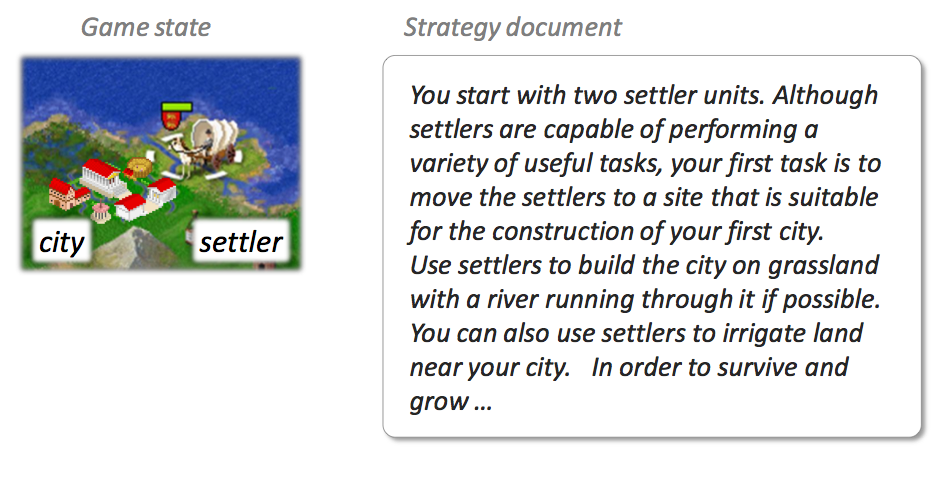
\includegraphics[width=\textwidth]{images/branavan-civ.png}}
\end{center}
\end{frame}

\begin{frame}\frametitle{FREECELL}
Eisenstein et al. 2009
\end{frame}

People:

RuleBased:
Winograd
Katz

SemParse:
Barzilay
Mooney
Zettlemoyer
Roth
Jordan

Lexical:
Siskind
Roy

Introduction

Natural language processing is a large field in the intersection of
linguistics (including phonology, morphology, syntax, semantics,
discourse, pragmatics), and computation (computability, complexity,
learnability).  This course will focus on aspects of NLP related to
extracting useful information from text (we will not talk about how we
get the text, e.g. speech recognition; or how we produce text,
e.g. natural language generation and summarization).  In particular we
will concentrate on methods that {\em learn} how to extract useful
information from text from given examples.  From a machine learning
perspective we imagine there is a function 

\[ f: X -> Y \]

which maps the input ($x \in X$ which in our case will be text), to an
output in a specified set $y \in Y$ and we would like to learn what
this function is by observing a number of $(x, y)$ examples ((this is
only supervised learning from annotated datasets)).  Typically the
mapping from $X$ to $Y$ may not be fully determined due to ambiguity,
missing information, etc.  In that case we will use a scoring function
as a target of our learning ((do we ever use f?))

\[ score: X x Y -> R \]

where $score(x, y)$ determines how good the output $y$ is for the
input $x$.  The score may or may not have a probabilistic
interpretation, and when it does we may choose to represent the joint
probability $p(x, y)$ or the conditional probability $p(y|x)$.
Working with probabilities have certain advantages ((what exactly)),
but require normalization (probabilities have to add to 1) which may
increase our computational cost ((why exactly are we paying this
price, what is wrong with unnormalized probabilities?)).  ((isn't all
this a bit too much detail before we give any examples of x and y?))
((how about unsupervised?))

The information extracted from text could be useful in and of itself
(sentiment analysis, spam detection), or part of a longer chain of
intermediate representations that we hope will lead to semantic
analysis (tagging, parsing).  We will categorize NLP problems based on
the complexity of the output:

\begin{itemize}
\item Text -> Label: spam detection, sentiment analysis, topic
  detection.
\item Text -> Probability: language modeling, with applications to
  lexical substitution, disambiguation.
\item Text (word sequence) -> Label sequence: tagging and chunking:
  POS, WSD, NER, NP chunking, morphological disambiguation.
\item Text (word sequence) -> Another word sequence: statistical
  machine translation.  The difference between this and labeling is
  (1) labeling is one-to-one, (2) monotonically ordered, (3) small
  vocabulary, none of which holds for SMT.
\item Text -> Trees: parsing, dependency, constituent, ccg.
\item Text -> Semantics: ((need to research this))
\end{itemize}

In machine learning terminology mapping inputs to discrete labels is
called classification, mapping inputs to numbers is called regression
and learning to estimate probabilities of a set of objects is called
density estimation.  Anything beyond that (starting with label
sequences) where the output has certain structure and components of
the output start to constrain and correlate with each other, is called
structured prediction.  ((give examples of e.g. postag interaction))

As the complexity of the output increases, so does the complexity of
learning and decoding (deciding on the best output).  Thus one way to
push the field forward is to investigate ways to learn and decode more
complex output sets.  Another way forward is to reduce the amount of
supervision and demonstrate learning where part or all of the examples
is missing their output (semisupervised and unsupervised learning), or
part of the input is missing (hidden variable learning).  ((How about
the example of using logic formulas vs just the answers in GeoQuery?
Knowing words vs trying to learn them from formulas?))


Datasets, References, and Examples

Many datasets for below tasks exist in nltk:
http://nltk.googlecode.com/svn/trunk/nltk_data/index.xml

1. CLASSIFICATION

Can we introduce generative, conditional, large margin, discriminative
etc. using this simple setting?  We can't introduce decoding though!

1.1 SPAM DETECTION
Ion Androutsopoulos got 500+ citations in a couple of papers:
http://www.aclweb.org/aclwiki/index.php?title=Spam_filtering_datasets
http://csmining.org/index.php/enron-spam-datasets.html
http://csmining.org/index.php/ling-spam-datasets.html
http://csmining.org/index.php/pu1-and-pu123a-datasets.html
http://csmining.org/index.php/spam-assassin-datasets.html
http://archive.ics.uci.edu/ml/datasets/Spambase: not good, already feature extracted

1.2 SENTIMENT ANALYSIS
The following paper introduced movie review data and got 2612 citations:
Bo Pang, Lillian Lee, and Shivakumar Vaithyanathan. Thumbs up? Sentiment classification using
machine learning techniques. In Proceedings of the Conference on Empirical Methods in Natural
Language Processing (EMNLP), pages 79–86, 2002.
- nltk uses this dataset for text classification example.
http://www.cs.cornell.edu/home/llee/opinion-mining-sentiment-analysis-survey.html
http://www.cs.cornell.edu/people/pabo/movie-review-data/
Thumbs up or thumbs down?: semantic orientation applied to unsupervised classification of reviews. PD Turney - Proceedings of the 40th annual meeting on association …, 2002 - dl.acm.org: Earlier paper, cited by Pang and Lee.


1.3 TEXT CLASSIFICATION
ir-book (2009) chap 13 is on classification: gives reuters, modapte split of reuters-21578 is standard, good review
manning chap 16 is on TC, uses reuters, explores different classification algorithms, introduces idtree, maxent, nb, perceptron, knn, does not mention svm, logistic regression
Top cited paper: McCallum1998 uses 5 datasets: Yahoo Science, Industry Sector, 20-newsgroups, webKB, Reuters-21578.
http://csmining.org/index.php/id-20-newsgroups.html
http://csmining.org/index.php/r52-and-r8-of-reuters-21578.html
http://qwone.com/~jason/20Newsgroups/
http://www.cs.cmu.edu/~TextLearning/datasets.html: has webkb, 20-newsgroups, industry-sector
/ai/data/nlp/reuters has both the old and new (rcv1) versions of reuters
http://www.ai.mit.edu/projects/jmlr/papers/volume5/lewis04a/lyrl2004_rcv1v2_README.htm -- standard ref for rcv1
jurafsky has nothing
This should lead to Blei2003 (LDA, cited 6708) and Teh2005 (HDP, cited 1362).  LDA uses TREC_AP corpus, scientific abstracts from C-elegans, compares with LSI, uses Reuters-21578 for dim reduction compares to all-words using Joachims1999 svmlight.  HDP uses C-elegans, NIPS articles with shared topics.  Compares infinite HMM with Stolcke-Omohundro bayesian model merging.

1.4 WORD CLUSTERING
isn't this close to unsupervised text classification?
Brown clusters use HMM.
How about LSA?  Can we go supervised text classification -> text clustering -> word clustering?
manning chap 14 is on clustering, 15.4 is on LSI, what is LSI vs LSA?
manning chap 15 is on IR, introduces vector space models, LSI, mentions Reuters (is introduced by Lewis 1992?)
DekangLin1998 also has stuff.

2. SLM
We can use the upos data (wsj)?
Can we do Turkish?  (would need morphologically split data, handling of unknowns etc.)
SRILM: [PDF] SRILM-an extensible language modeling toolkit. A Stolcke - INTERSPEECH, 2002 - (2502 citations)
An empirical study of smoothing techniques for language modeling. SF Chen, J Goodman - Proceedings of the 34th annual meeting on …, 1996 - cited by 1411, but the following is more informative:
A bit of progress in language modeling JT Goodman - Computer Speech & Language, 2001 - Elsevier (395 citations)
He used NAB:
All of our experiments were performed on the NAB (North American Business news) corpus (Stern, 1996). We performed most experiments at 4 different
training data sizes: 100,000 words, 1,000,000 words, 10,000,000 words, and the
whole corpus – except 1994 WSJ data – approximately 284,000,000 words. In
all cases, we performed parameter optimization on a separate set of heldout
data, and then performed testing on a set of test data. None of the three data
sets overlapped. The heldout and test sets were always every fiftieth sentence
from two non-overlapping sets of 1,000,000 words, taken from the 1994 section.
  We also have:
Two decades of statistical language modeling: Where do we go from here?  R Rosenfeld - Proceedings of the IEEE, 2000 - ieeexplore.ieee.org
An empirical study of smoothing techniques for language modeling. SF Chen, J Goodman - Computer Speech & Language, 1999 - Elsevier
A hierarchical Bayesian language model based on Pitman-Yor processes.  YW Teh - Proceedings of the 21st International Conference on …, 2006 - dl.acm.org
Improved backing-off for m-gram language modeling.  R Kneser, H Ney - … , and Signal Processing, 1995. ICASSP-95., …, 1995 - ieeexplore.ieee.org

3. TAGGING AND CHUNKING

3.1 NP CHUNKING 
- conll 1999-2000

3.2 NER
- conll 2002-2003

3.3 POS
- PTB WSJ
Feature-rich part-of-speech tagging with a cyclic dependency network. K Toutanova, D Klein, CD Manning… - Proceedings of the 2003 …, 2003 - dl.acm.org
[PDF] A maximum entropy model for part-of-speech tagging.  A Ratnaparkhi - Proceedings of the conference on empirical …, 1996 - acl.ldc.upenn.edu

3.4 MOR
- My dataset?
Two-level description of Turkish morphology.  K Oflazer - Literary and linguistic computing, 1994 - ALLC
Dependency parsing of Turkish. G Eryiğit, J Nivre, K Oflazer - Computational Linguistics, 2008 - MIT Press
Finite State Morphology textbook.
Xerox tools and its free versions?
Need to talk about FST if we are going to learn it:
Stolcke and Omohundro, Xavier Carreras, HDP paper etc.
Morphochallenge?
Disambiguation just tagging but learning anything else goes deeper.

3.5 WSD
- Semeval?

4. SMT
Sentence alignment: Gale and Church 1993
Word alignment: Brown 1990
Check out Noah 1.9, 1.10.

5. PARSING

5.1 PS-PARSING
- PTB WSJ, standard split
Building a large annotated corpus of English: The Penn Treebank.  MP Marcus, MA Marcinkiewicz, B Santorini - Computational linguistics, 1993 - dl.acm.org
Study Charniak, Collins, Stanford, and Berkeley models?
A maximum-entropy-inspired parser. E Charniak - Proceedings of the 1st North American chapter of the …, 2000 - dl.acm.org
Head-driven statistical models for natural language parsing.  M Collins - Computational linguistics, 2003 - MIT Press
Accurate unlexicalized parsing.  D Klein, CD Manning - Proceedings of the 41st Annual Meeting on …, 2003 - dl.acm.org
Petrov and Klein: which reference?  Noah says 2008.
de Marnffe and Manning: Stanford typed dependencies
Unsupervised?  Rens Bod?  DMV, CCM?
TAG?  TSG?

5.2 DEP-PARSING
- conll 2006-2007
Dependency parsing of Turkish. G Eryiğit, J Nivre, K Oflazer - Computational Linguistics, 2008 - MIT Press
MaltParser: A language-independent system for data-driven dependency parsing.  J Nivre, J Hall, J Nilsson, A Chanev… - Natural Language …, 2007 - Cambridge Univ Press
Non-projective dependency parsing using spanning tree algorithms. R McDonald, F Pereira, K Ribarov, J Hajič

5.3 CCG-PARSING
Clark and Curran 2004: CCG parser
Carreras, Collins, Koo 2008: TAG parsing
Riezler 2000: constraint based?

6. SEMANTIC PARSING
- GeoQuery: Zelle and Mooney 1996, Wong and Mooney 2007, Zettlemoyer and Collins 2005, Clarke and Goldwasser 2010, Liang-Jordan-Klein-2011/2013
- Robot: Ge and Mooney 2005
- Travel: Mooney 1997
- Vision

0. SRL
which math?
conll 2004, 2005
Automatic labeling of semantic roles.  D Gildea, D Jurafsky - Computational linguistics, 2002 - MIT Press
The proposition bank: An annotated corpus of semantic roles. M Palmer, D Gildea, P Kingsbury - Computational Linguistics, 2005 - MIT Press


0. COREF
which math?
conll 2011, 2012
Ng and Cardie 2002
Culotta, McCallum 2007
Haghighi, Klein 2009
Poon, Domingos 2008

Introduce WordNet (Fellbaum1998) and Celex?
ConceptNet, PropBank (Palmer2005), FrameNet (Baker1998), NomBank, Ontonotes?
Discourse treebank (Carlson2003), Discourse graphbank (Wolf2005), Penn Discourse treebank (Prasad2008), Discourse tutorial (Webber2010)
Concentrate on learning not problems and resources!

From Noah review by Quirk: It is a comprehensive introduction to the most common and effective decoding
approaches, with one significant exception: the recent advances in dual decomposition
and Lagrangian relaxation methods. Timing is likely the culprit. This book was developed mainly from 2006 to 2009, whereas dual decomposition did not attain notoriety in
our community until a few years later (Rush et al. 2010). Relaxation approaches, though
potentially a passing phase, have successfully broadened the reach of simpler decoding
techniques into more complicated domains such as structured event extraction.

Hard EM is mentioned in the context
of several examples, though a more detailed description of this potentially important
technique (cf. Spitkovsky et al., 2010) would bridge the material of Chapters 2 and 4.

\end{document}
